\chapter{Methodology}
\section{Threat Modeling}
Threat modeling is a technique that allows us to detect and address top threats that can have a significant impact on the application \citep{threat_modeling}. Similarly, this web application uses the STRIDE threat model to discover threats. This model is used as it is one of the most mature threat analysis methods adopted by Microsoft \citep[p.~1]{shevchenko2018threat}. Similarly, this web application uses the STRIDE threat model to discover threats. The threats listed in the table will be tested against the system to detect if the vulnerabilities exist.
Using the DFD (see figure \ref{fig:dfd}), we can list out some threats using the STRIDE (Spoofing, Tampering, Redupation, Information Disclosure, Denial of Service, and Elevation of Privilege) \citep[p.~2]{stride}.

\begingroup
\centering
\setlength{\tabcolsep}{6.5pt} % Default value: 6pt
\renewcommand{\arraystretch}{1.8} % Default value: 1
\begin{longtable}{ |p{7cm}| p{8cm} |}
\caption{STRIDE Modeling}
    \label{table:spoofing}
\hline
\rowcolor{grey!15}
\textbf{STRIDE} & \textbf{Threats}\\
\hline
Spoofing & \begin{enumerate}
    \item DNS spoofing allowing to redirect to a malicious site.
    \item Ip Spoofing \citep[p.~2]{ip_spoofing}
\end{enumerate} \\
\hline
Tampering & \begin{enumerate}
    \item Upload malicious files.
    \item Cross-Site Request Forgery. \citep[p.~538]{crsf}
\end{enumerate} \\
\hline
Repudiation & \begin{enumerate}
    \item Malicious activities are not tracked.
\end{enumerate} \\
\hline
Information Disclosure & \begin{enumerate}
    \item SQL Injection into the database.
    \item Various network information is public.
\end{enumerate} \\
\hline
Denial of Service & \begin{enumerate}
    \item The CMS site is hit with a DoS attack.
\end{enumerate} \\
\hline
Elevation of Privileges & \begin{enumerate}
    \item Unauthorized users with admin privileges are added.
\end{enumerate} \\
\hline
\end{longtable}
\endgroup

\begin{figure}[h!]
\centering
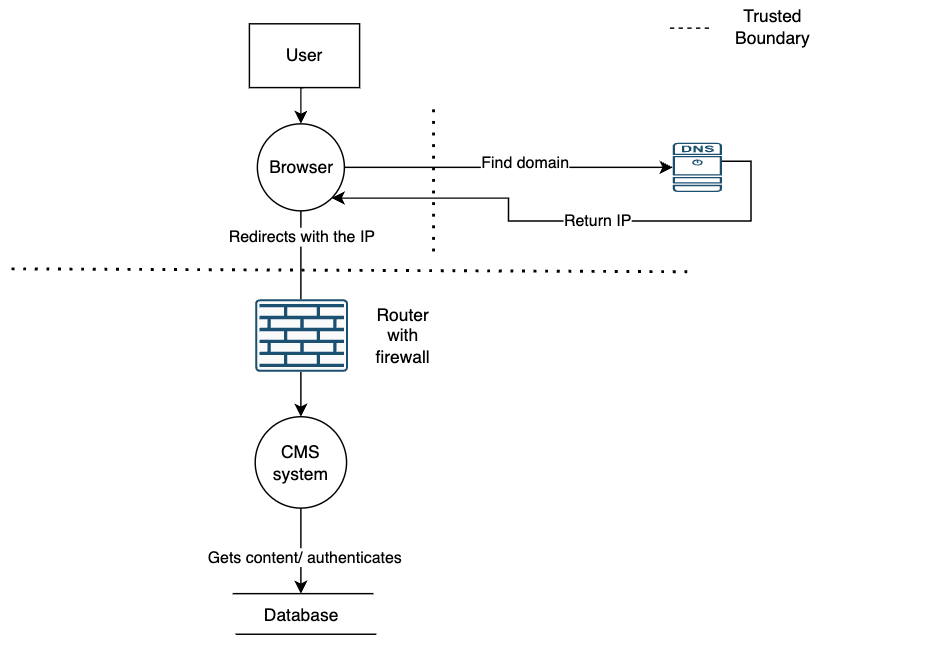
\includegraphics[width=\textwidth, height=450px]{pics/dfd.png}
\caption{DFD level 0 for the CMS system}\label{fig:dfd}
\end{figure}


\section{Vulnerability Assessment}
For the vulnerability assessment, the automated tools (see table \ref{table:tools}) mentioned in the baseline analysis were used to scan for known threats and misconfigurations of the CMS system using the adversary behaviors defined in MITRE Enterprise ATT\&CK matrix \citep[p.~158]{xiong2022cyber}.

\begin{comment}
Additionally, the assessment and reconnaissance are performed using the MITRE Enterprise ATT\&CK matrix \citep{mitre_url}, as this model describes the adversary behaviors that measure the system's resilience at an enterprise level \citep[p.~158]{xiong2022cyber}.
\end{comment}


\newpage
\begingroup
\centering
\setlength{\tabcolsep}{6.5pt} % Default value: 6pt
\renewcommand{\arraystretch}{1.8} % Default value: 1
\begin{longtable}{ |p{5cm}| p{10cm} |}
\caption{Results from the tools used in the assessment}
    \label{table:tools}
\hline
\rowcolor{grey!15}
\textbf{Tool}  & \textbf{Result}\\
\hline
Cmsmap &  \begin{enumerate}
    \item CMS Detected version detected.
    \item PHP version detected.
\end{enumerate}\\
\hline
Metasploit \& Nmap &  \begin{enumerate}
    \item Discovered network misconfigurations.
    \item Tested against major CRM threats (i.e., SQL injection, XSS, RCE, Directory traversal) mentioned in the baseline analysis.
\end{enumerate}\\
\hline
DNSrecon &  \begin{enumerate}
    \item Performed reverse lookup and CDN detection.
    \item Performed DNS Zone transfer.
    \item Performed Cache Snooping and DNS Recursion.
    \item Performed Zone walking.
\end{enumerate}\\
\hline
\end{longtable}
\endgroup